\section{Actividad No 05 – Funciones}
	
\begin{enumerate}[1.]
	\item Se requiere realizar una consulta que visualice la fecha del sistema.
	\\
	\\SELECT CONVERT (date, SYSDATETIME())
	\\,CONVERT (date, SYSDATETIMEOFFSET())
	\\,CONVERT (date, SYSUTCDATETIME())
	\\,CONVERT (date, CURRENT\_TIMESTAMP)
	\\,CONVERT (date, GETDATE())
    	\\,CONVERT (date, GETUTCDATE());
	\begin{center}
	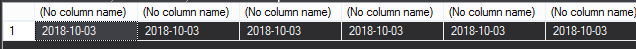
\includegraphics[width=5cm]{./Imagenes/451}
	\end{center}
	
	\item El departamento de Recursos Humanos necesita un reporte de todos los empleados que muestre el No de Empleado, Apellidos, Salario y una columna más con el cálculo del salario incrementado en 15.5\% (expresado solo en enteros) esta columna debe etiquetarse Nuevo Salario
	\\
	\\SELECT employee\_id,last\_name,salary,salary*0.155 as newsalary FROM employees
	\begin{center}
	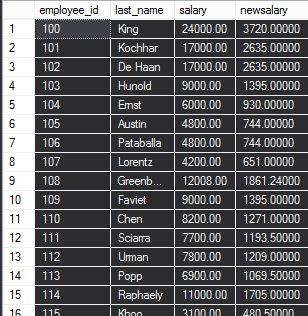
\includegraphics[width=5cm]{./Imagenes/452}
	\end{center}

	\item Modificar la consulta anterior y adicionar una columna que muestre el resultado de la resta entre el antiguo salario y el nuevo salario. Etiquetar esta columna como Incremento.
	\\
	\\SELECT employee\_id,last\_name,salary,salary*0.155 as newsalary,salary-(salary*0.155) as incremento FROM employees
	\begin{center}
	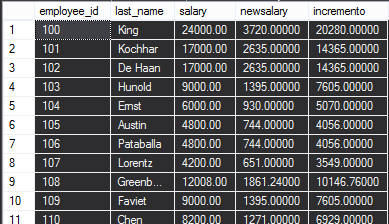
\includegraphics[width=5cm]{./Imagenes/453}
	\end{center}

	\item Crear un reporte que muestre los Apellidos (con la primera letra en May\'usculas y las demás en Min\'usculas) y la longitud de los apellidos (colocar alias Longitud), para todos aquellos empleados quienes sus apellidos empiecen con las letras ‘J’, ‘A’ y ‘M’. Ordenar los resultados por la columna Apellido.
	\\
	\\select UPPER(last\_name) "Apellido", (LOWER(first\_name)) "Longitud" 
	\\from employees 
	\\where last\_name like 'A\%'
     	\\ or last\_name like 'J\%'
      	\\or last\_name like 'M\%' order by last\_name asc;
      	\begin{center}
	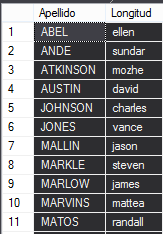
\includegraphics[width=5cm]{./Imagenes/454}
	\end{center}

	\item Modificar la consulta anterior a fin de que consulte primero al usuario con que letra empieza el apellido a buscar. Considerar que no importa si la letra esta may\'uscula o min\'uscula de igual manera debe mostrar los resultados.
	\\
	\\select initcap(FIRST\_NAME) as "name", length(first\_name) as "Length" from employees where upper(substr(first\_name,1,1))=upper('\&Inicial') order by first\_name;

	\item El departamento de Recursos Humanos la duración o tiempo de permanencia de cada empleado, mostrar el Apellido y el calculo del número de meses entre la fecha de hoy y la fecha en que fue contratado el empleado, Etiquetar la columna como Meses Trabajados, ordenar los resultados por el resultado de los n\'umeros de meses, Redondear el número de meses al entero más cercano.
	\\
	\\SELECT LAST\_NAME, ROUND(MONTHS\_BETWEEN(SYSDATE,HIRE\_DATE),0) "MONTHS\_WORKED"
	\\from employees order by MONTHS\_BETWEEN( HIRE\_DATE, SYSDATE);

	\item Crear una consulta que devuelva los Apellidos y Salarios de todos los empleados, Formatear la columna salario para que muestre 15 caracteres, completar con el símbolo ‘\$’ los espacios previos al valor de la columna salario, ejemplo: \$\$\$\$\$\$\$\$\$\$10000. Etiquetar esta columna como Salario.
	\\
	\\CREATE FUNCTION LPAD
	\\(
	\\ @string VARCHAR(MAX), 
	\\@length INT,          
	\\@pad CHAR             
	\\)
	\\RETURNS VARCHAR(MAX)
	\\AS
	\\BEGIN
	    \\RETURN REPLICATE(@pad, @length - LEN(@string)) + @string;
	\\END
	\\GO
	\\SELECT dbo.LPAD(salary, 15, '\$') VALUE
	\\FROM employees;
	\begin{center}
		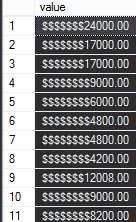
\includegraphics[width=5cm]{./Imagenes/457}
	\end{center}

	\item Crear una consulta que muestre en una única columna los primeros 8 caracteres del apellido de los empleados e indique sus salarios representados por asteriscos (‘*’), cada asterisco representa el valor 1000. Ordenar el listado por el salario de los empleados. Asimismo Etiquetar la columna como ‘Empleados y sus Salarios’.
	\item Finalmente crear una consulta que muestre los Apellidos de los empleados y el No de Semanas Empleado hasta la actualidad para todos los empleados del departamento No 90, truncar el número de semanas a sin decimales. Ordenar el resultado por el No de Semanas y etiquetar la columna como tenencia.
	\\
	\\select last\_name, TRUNC(((SYSDATE-hire\_date)/7),0) as TENURE from employees where department\_id=90 ORDER BY hire\_date DESC;
\end{enumerate}

